%!TEX root = ../Osteuropaatlas.tex

\section{Wirtschaftliche Strukturdaten}


\setcounter{figure}{1}
\begin{figure}[!h]
	\addcontentsline{toc}{subsection}{IMD Wirtschaftsleistungsranking}
	\caption{IMD Wirtschaftsleistungsranking}
	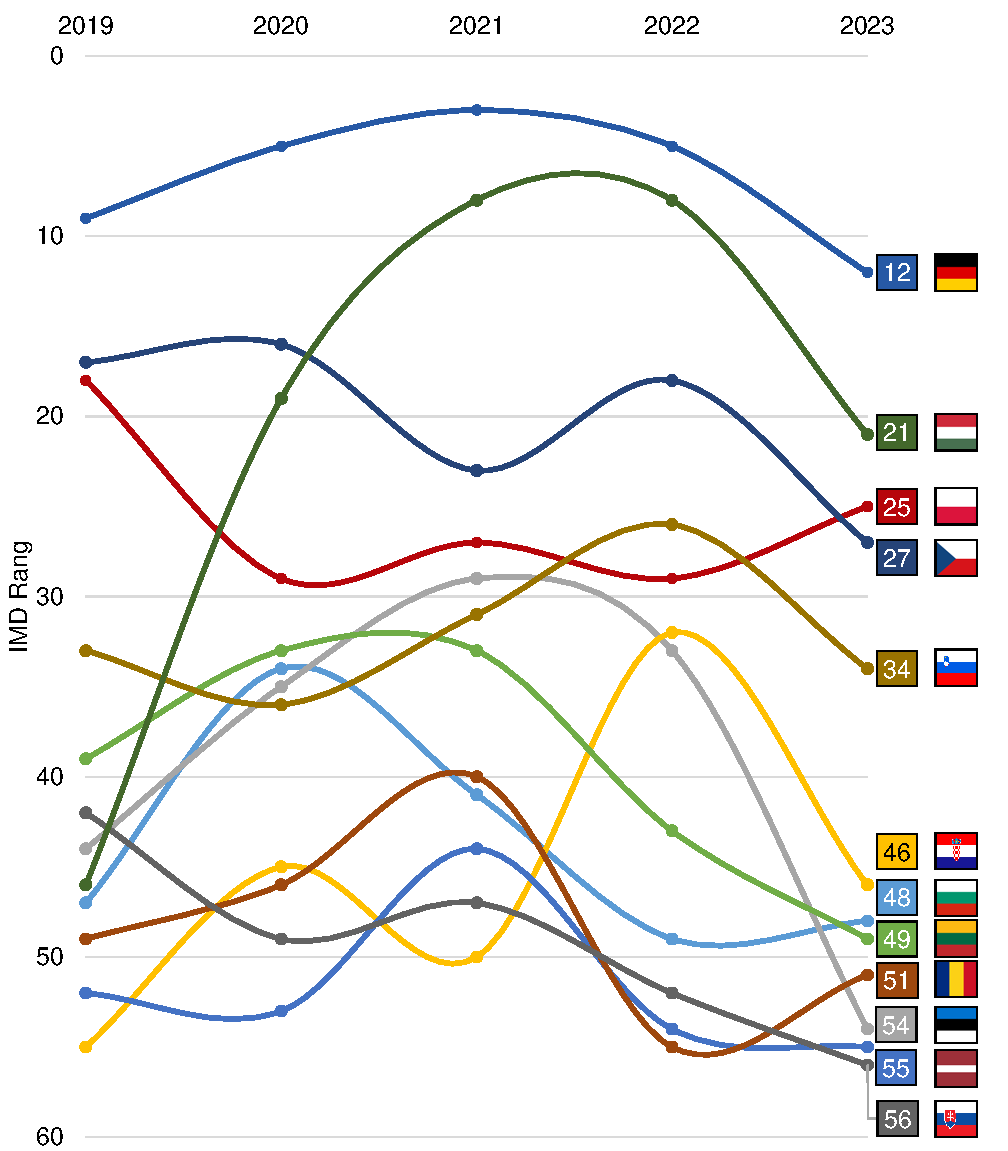
\includegraphics[width = \textwidth, height = 19.5cm]{IMD_Ranking}
	\begin{spacing}{1} \scriptsize
		\vspace{2mm}
		Anm.: IMD Economic Performance Ranking; Stand 2023\\
		Quelle: IMD World Competitiveness Center (2024); Dar. imreg (2024) \end{spacing}
\end{figure}


\begin{figure}[p]
	\addcontentsline{toc}{subsection}{Arbeitsstunden}
	{\centering \maps{Arbeitsstunden}}
	\label{map:stundengeleistet}
	\karte{Arbeitsstunden_geleistet}{2020}{Veränderung 2015 bis 2020}
	\begin{spacing}{1} \scriptsize
		Anm.: Jährliche Summe geleisteter Arbeitsstunden unabhängig von Bezahlung; Stand 2020\\
		Quelle: Eurostat (2024); Ber. \& Dar. imreg (2024) \end{spacing}
\end{figure}


\begin{figure}[p]
	\addcontentsline{toc}{subsection}{Arbeitsstunden je Erwerbstätigen}
	{\centering \maps{Arbeitsstunden je Erwerbstätigen}}
	\label{map:stundengeleistetprokopf}
	\karte{Arbeitsstunden_proErwerbstaetigen}{2020}{Veränderung 2015 bis 2020}
	\begin{spacing}{1} \scriptsize
		Anm.: Jährliche Summe geleisteter Arbeitsstunden unabhängig von Bezahlung; Stand 2020\\
		Quelle: Eurostat (2024); Ber. \& Dar. imreg (2024) \end{spacing}
\end{figure}


\begin{figure}[p]
	\addcontentsline{toc}{subsection}{Arbeitnehmerentgelt}
	{\centering \maps{Arbeitnehmerentgelt}}
	\label{map:entgelt}
	\karte{Arbeitnehmerentgelt}{2020}{Veränderung 2015 bis 2020}
	\begin{spacing}{1} \scriptsize
		Anm.: Jährliche Entgeltsumme; Stand 2020\\
		Quelle: Eurostat (2024); Ber. \& Dar. imreg (2024) \end{spacing}
\end{figure}


\begin{figure}[p]
	\addcontentsline{toc}{subsection}{Arbeitnehmerentgelt je Arbeitnehmer}
	{\centering \maps{Arbeitnehmerentgelt je Arbeitnehmer}}
	\label{map:entgeltprokopf}
	\karte{Entgelt_proKopf}{2020}{Veränderung 2015 bis 2020}
	\begin{spacing}{1} \scriptsize
		Anm.: Jährliche Entgeltsumme; Stand 2020\\
		Quelle: Eurostat (2024); Ber. \& Dar. imreg (2024) 
	\end{spacing}
\end{figure}


\begin{figure}[p]
	\addcontentsline{toc}{subsection}{Arbeitnehmerentgelt je Arbeitsstunde}
	{\centering \maps{Arbeitnehmerentgelt je Arbeitsstunde}}
	\label{map:entgeltprostunde}
	\karte{Entgelt_proH}{2020}{Veränderung 2015 bis 2020}
	\begin{spacing}{1} \scriptsize
		Anm.: Jährliche Entgeltsumme; Stand 2020\\
		Quelle: Eurostat (2024); Ber. \& Dar. imreg (2024) 
	\end{spacing}
\end{figure}


\begin{figure}[p]
	\addcontentsline{toc}{subsection}{Arbeitproduktivität je Erwerbestätigen (nominal)}
	{\centering \maps{Arbeitproduktivität je Erwerbestätigen (nominal)}}
	\label{map:prodprokopfnom}
	\karte{Arbeitsproduktivitaet_proErwerbstaetigen_nom}{2020}{Veränderung 2015 bis 2020}
	\begin{spacing}{1} \scriptsize
		Anm.: Jährlicher nominaler Produktionswert je Erwerbstätigen; Stand 2020\\
		Quelle: Eurostat (2024); Ber. \& Dar. imreg (2024) 
	\end{spacing}
\end{figure}


\begin{figure}[p]
	\addcontentsline{toc}{subsection}{Arbeitproduktivität je Arbeitsstunde (nominal)}
	{\centering \maps{Arbeitproduktivität je Arbeitsstunde (nominal)}}
	\label{map:prodprostundenom}
	\karte{Arbeitsproduktivitaet_proH_nom}{2020}{Veränderung 2015 bis 2020}
	\begin{spacing}{1} \scriptsize
		Anm.: Jährlicher nominaler Produktionswert je Arbeitsstunde; Stand 2020\\
		Quelle: Eurostat (2024); Ber. \& Dar. imreg (2024) 
	\end{spacing}
\end{figure}


\begin{figure}[p]
	\addcontentsline{toc}{subsection}{Entwicklung Arbeitsproduktivität (real)}
	{\centering \maps{Entwicklung Arbeitsproduktivität (real)}}
	\label{map:bipvol}
	\makebox[\linewidth][c]{
		\begin{subfigure}{0.61\textwidth}
			\centering
			\caption{Arbeitproduktivität je Erwerbestätigen (real)\\Veränderung 2015 bis 2020}
			\includegraphics[width=\textwidth, height=172mm, center]{Arbeitsproduktivitaet_proErwerbstaetigen_real_Delta} 
		\end{subfigure}
		\begin{subfigure}{0.61\textwidth}
			\centering
			\caption{Arbeitproduktivität je Arbeitsstunde (real)\\Veränderung 2015 bis 2020}
			\includegraphics[width=\textwidth, height=172mm, center]{Arbeitsproduktivitaet_proH_real_Delta}
		\end{subfigure}
	}
	\begin{spacing}{1} \scriptsize
		Anm.: Jährlicher nominaler Produktionswert je Erwerbestätigen/Arbeitsstunde Stand 2020\\
		Quelle: Eurostat (2024); Ber. \& Dar. imreg (2024) \end{spacing}
\end{figure}


\begin{figure}[p]
	\addcontentsline{toc}{subsection}{Anlageninvestitionen}
	{\centering \maps{Anlageninvestitionen}}
	\label{map:invest}
	\karte{Anlageninvestition}{2020}{Veränderung 2015 bis 2020}
	\begin{spacing}{1} \scriptsize
		Anm.: Anlageninvestitionen; Stand 2020\\
		Quelle: Eurostat (2024); Ber. \& Dar. imreg (2024) 
	\end{spacing}
\end{figure}


\begin{figure}[p]
	\addcontentsline{toc}{subsection}{Anzahl Unternehmen im Verarbeitenden Gewerbe}
	{\centering \maps{Anzahl Unternehmen im Verarbeitenden Gewerbe}}
	\label{map:unternehmenvg}
	\karte{StrukturVG_UntZahl}{2020}{Veränderung 2015 bis 2020}
	\begin{spacing}{1} \scriptsize
		Anm.: Stand 2020\\
		Quelle: Eurostat (2024); Ber. \& Dar. imreg (2024) 
	\end{spacing}
\end{figure}


\begin{figure}[p]
	\addcontentsline{toc}{subsection}{Anzahl Beschäftigter im Verarbeitenden Gewerbe}
	{\centering \maps{Anzahl Beschäftigter im Verarbeitenden Gewerbe}}
	\label{map:beschvg}
	\karte{StrukturVG_BeschZahl}{2020}{Veränderung 2015 bis 2020}
	\begin{spacing}{1} \scriptsize
		Anm.: Stand 2020\\
		Quelle: Eurostat (2024); Ber. \& Dar. imreg (2024) 
	\end{spacing}
\end{figure}


\begin{figure}[p]
	\addcontentsline{toc}{subsection}{Anteil Beschäftigter im Verarbeitenden Gewerbe an allen Beschäftigten}
	{\centering \maps{Anteil Beschäftigter im Verarbeitenden Gewerbe an allen Beschäftigten}}
	\label{map:beschanteilvg}
	\karte{Beschaeftigungsanteil_VG}{2022}{Veränderung 2015 bis 2022}
	\begin{spacing}{1} \scriptsize
		Anm.: Stand 2022\\
		Quelle: Eurostat (2024); Ber. \& Dar. imreg (2024) 
	\end{spacing}
\end{figure}


\begin{figure}[p]
	\addcontentsline{toc}{subsection}{Arbeitsstunden im Verarbeitenden Gewerbe}
	{\centering \maps{Arbeitsstunden im Verarbeitenden Gewerbe}}
	\label{map:stundengeleistetvg}
	\karte{Arbeitsstunden_geleistetVG}{2020}{Veränderung 2015 bis 2020}
	\begin{spacing}{1} \scriptsize
		Anm.: Jährliche Summe geleisteter Arbeitsstunden unabhängig von Bezahlung; Stand 2020\\
		Quelle: Eurostat (2024); Ber. \& Dar. imreg (2024) \end{spacing}
\end{figure}


\begin{figure}[p]
	\addcontentsline{toc}{subsection}{Arbeitnehmerentgelt im Verarbeitenden Gewerbe}
	{\centering \maps{Arbeitnehmerentgelt im Verarbeitenden Gewerbe}}
	\label{map:entgeltvg}
	\karte{Arbeitnehmerentgelt_VG}{2020}{Veränderung 2015 bis 2020}
	\begin{spacing}{1} \scriptsize
		Anm.: Jährliche Entgeltsumme; Stand 2020\\
		Quelle: Eurostat (2024); Ber. \& Dar. imreg (2024) \end{spacing}
\end{figure}

\begin{figure}[p]
	\addcontentsline{toc}{subsection}{Lohn \& Gehalt im Verarbeitenden Gewerbe}
	{\centering \maps{Lohn \& Gehalt im Verarbeitenden Gewerbe}}
	\label{map:entgeltvg2}
	\karte{StrukturVG_Lohn}{2020}{Veränderung 2015 bis 2020}
	\begin{spacing}{1} \scriptsize
		Anm.: Jährliche Lohn- \& Gehaltssumme; Stand 2020\\
		Quelle: Eurostat (2024); Ber. \& Dar. imreg (2024) \end{spacing}
\end{figure}


\begin{figure}[p]
	\addcontentsline{toc}{subsection}{Arbeitnehmerentgelt je Arbeitsstunde im Verarbeitenden Gewerbe}
	{\centering \maps{Arbeitnehmerentgelt je Arbeitsstunde im Verarbeitenden Gewerbe}}
	\label{map:entgeltprostundevg}
	\karte{Entgelt_proHVG}{2020}{Veränderung 2015 bis 2020}
	\begin{spacing}{1} \scriptsize
		Anm.: Jährliche Entgeltsumme; Stand 2020\\
		Quelle: Eurostat (2024); Ber. \& Dar. imreg (2024) 
	\end{spacing}
\end{figure}


\begin{figure}[p]
	\addcontentsline{toc}{subsection}{Anlageninvestitionen im Verarbeitenden Gewerbe}
	{\centering \maps{Anlageninvestitionen im Verarbeitenden Gewerbe}}
	\label{map:investvg}
	\karte{AnlageninvestitionVG}{2020}{Veränderung 2015 bis 2020}
	\begin{spacing}{1} \scriptsize
		Anm.: Anlageninvestitionen; Stand 2020\\
		Quelle: Eurostat (2024); Ber. \& Dar. imreg (2024) 
	\end{spacing}
\end{figure}


\begin{figure}[p]
	\addcontentsline{toc}{subsection}{Investitionsintensität im Verarbeitenden Gewerbe}
	{\centering \maps{Investitionsintensität im Verarbeitenden Gewerbe}}
	\label{map:investintenvg}
	\karte{InvestitionsintensitaetVG}{2020}{Veränderung 2015 bis 2020}
	\begin{spacing}{1} \scriptsize
		Anm.: Anlageninvestitionen je Beschäftigten; Stand 2020\\
		Quelle: Eurostat (2024); Ber. \& Dar. imreg (2024) 
	\end{spacing}
\end{figure}

